As a contribution for this work, we propose realizing the \textsc{Forager} toolkit as a usable software package and system for individual use. We project an initial release of this software by June 2023. System progress and planned development can be viewed in the Gantt chart in Figure~\ref{fig:gantt}. The final deliverable of this system will be a command line interface (CLI) application installed through PyPi. We will provide the following components in the initial release.

\textbf{TaPcap: } This option will parse input PCAP files, extracting header features and/or payloads into CSV or text file format.

\textbf{\textsc{TRex}: } This option will find frequent tokens according to a provided threshold from a CSV output from \textsc{TaPcap}.

\textbf{\textsc{GRex}: } This option will perform genetic sequencing alignment of payloads from a CSV output from \textsc{TaPcap}.

\textbf{\textsc{Alpine}: } In training mode, this model will accept as input the CSV obtained from \textsc{TaPcap}, generate locality sensitive hashes from the header data, and finalize and serialize these to an LSHForest~\cite{lshforest}. In testing mode, the trained LSHForest will be reloaded. Locality sensitive hashes of the input data will be generated and index lookup performed. The returned result will be applied to the ensemble voting system if other models are configured.

\textbf{\textsc{Palm}: } In training mode, this model will accept as input the CSV obtained from \textsc{TaPcap}, generate locality sensitive hashes from the payload data, and finalize and serialize these to an LSHForest~\cite{lshforest}. In testing mode, the trained LSHForest will be reloaded. Locality sensitive hashes of the input data will be generated and index lookup performed. The returned result will be applied to the ensemble voting system if other models are configured.

\textbf{\textsc{Maple}: } In training mode, this model will accept as input the CSV obtained from \textsc{TaPcap}, generate grayscale images from the payload data, and save the generated neural network model and trained weights to JSON and H5 files, respectively. In testing mode, the trained neural network will be reloaded. Grayscale images of the input data will be generated and used as input to the CNN classifier. The returned result will be applied to the ensemble voting system if other models are configured.

\textbf{\textsc{Date}: } In training mode, this model will accept as input the CSV obtained from \textsc{TaPcap}, generate point clouds from the payload data and perform DBSCAN analysis, and save the generated neural network model and trained weights to JSON and H5 files, respectively. In testing mode, the trained neural network will be reloaded. Point clouds will be generated from input data and DBSCAN analysis performed, and this will be used as input to the multi-layer perceptron classifier. The returned result will be applied to the ensemble voting system if other models are configured.

\textbf{Multi-modality: } \textsc{Forager} will support using one or more of the \textsc{Alpine}, \textsc{Palm}, \textsc{Maple}, and \textsc{Date} models together so that the packet may be analyzed from multiple representations. We will use votes in a combined ensemble classifier and return the index with the most votes as the classification.

\textbf{Tagging: } \textsc{Forager} will write the classification to a column in the \textsc{TaPcap} file.

\begin{figure*}
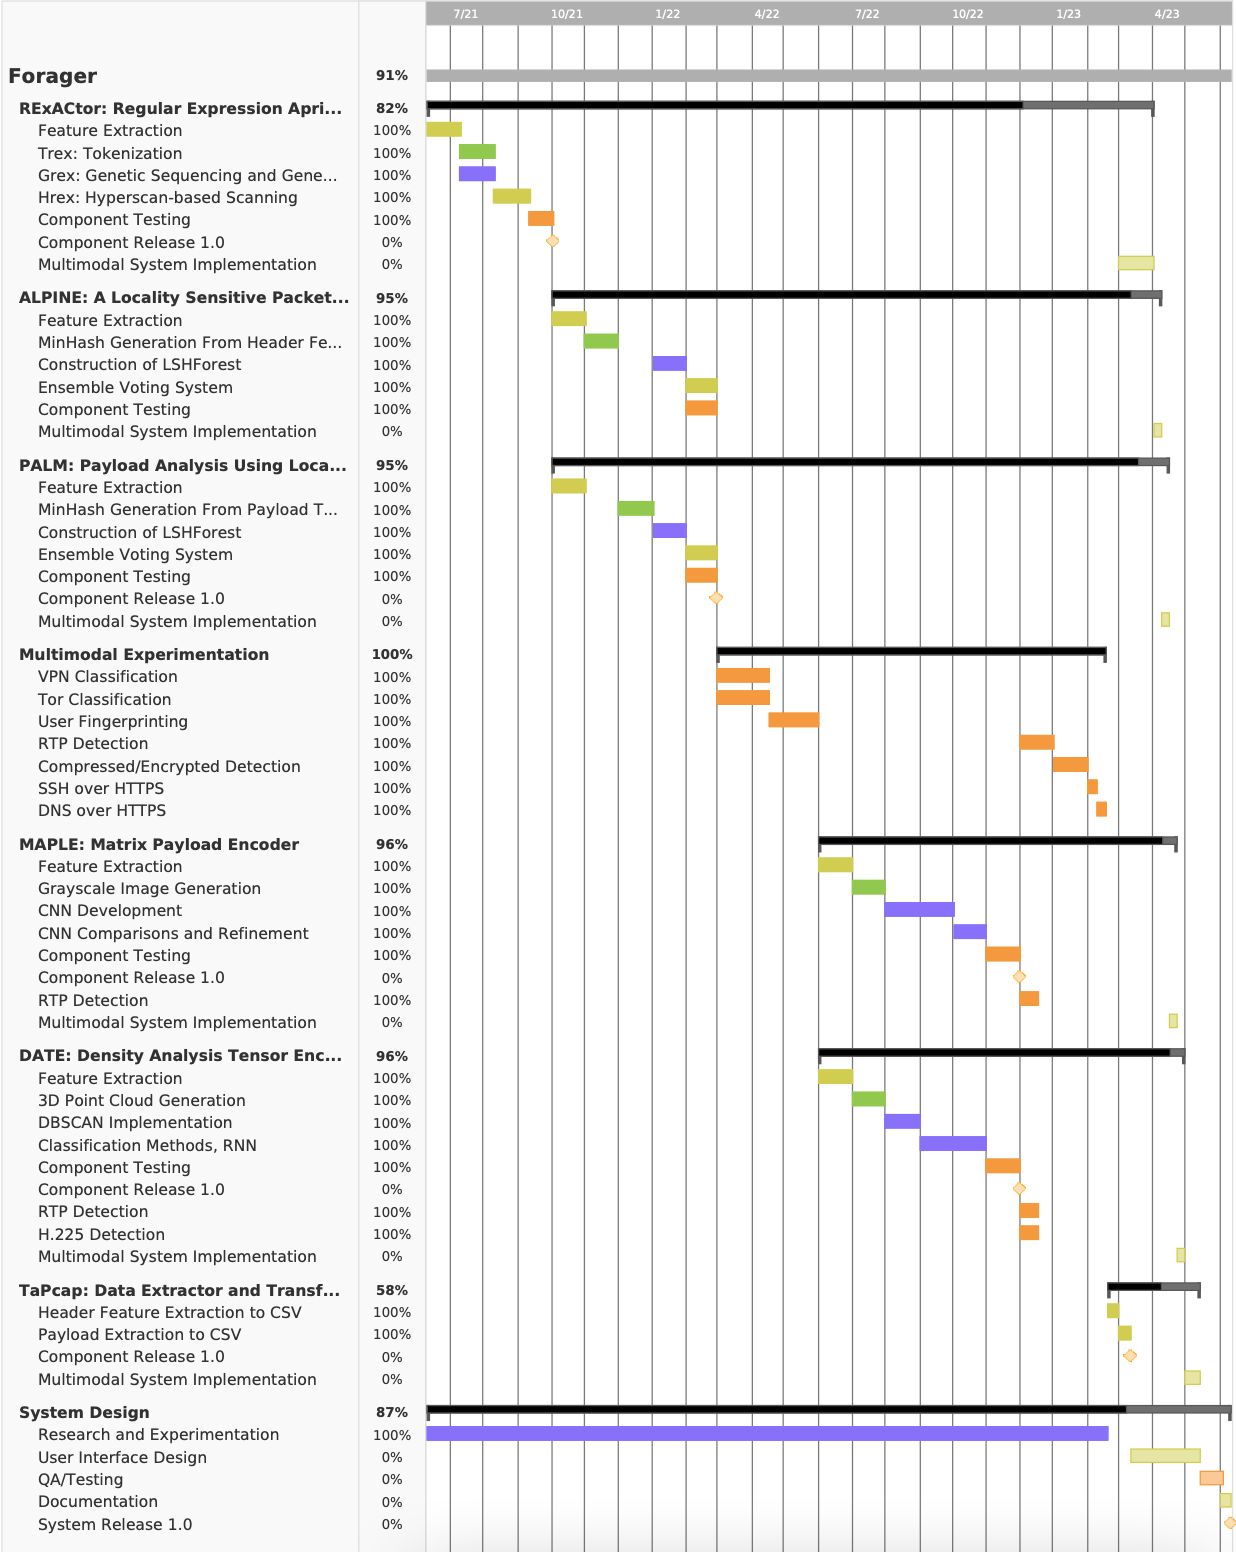
\includegraphics[width=\textwidth,height=\textheight]{chapters/expected/img/gantt.png}
\caption{Gantt chart of \textsc{Forager} 1.0.}
\label{fig:gantt}
\end{figure*}
